\section{Problem Description}\label{sec:problemDescription}

The system is underactuated, and nonlinear.

%The system in \autoref{fig:system}, is the well-known cart pendulum system. The system can only be controlled by a the force shown directly on the cart in the horisontal direction. So the system is underactuated, and nonlinear.

%\begin{figure}[H]
%  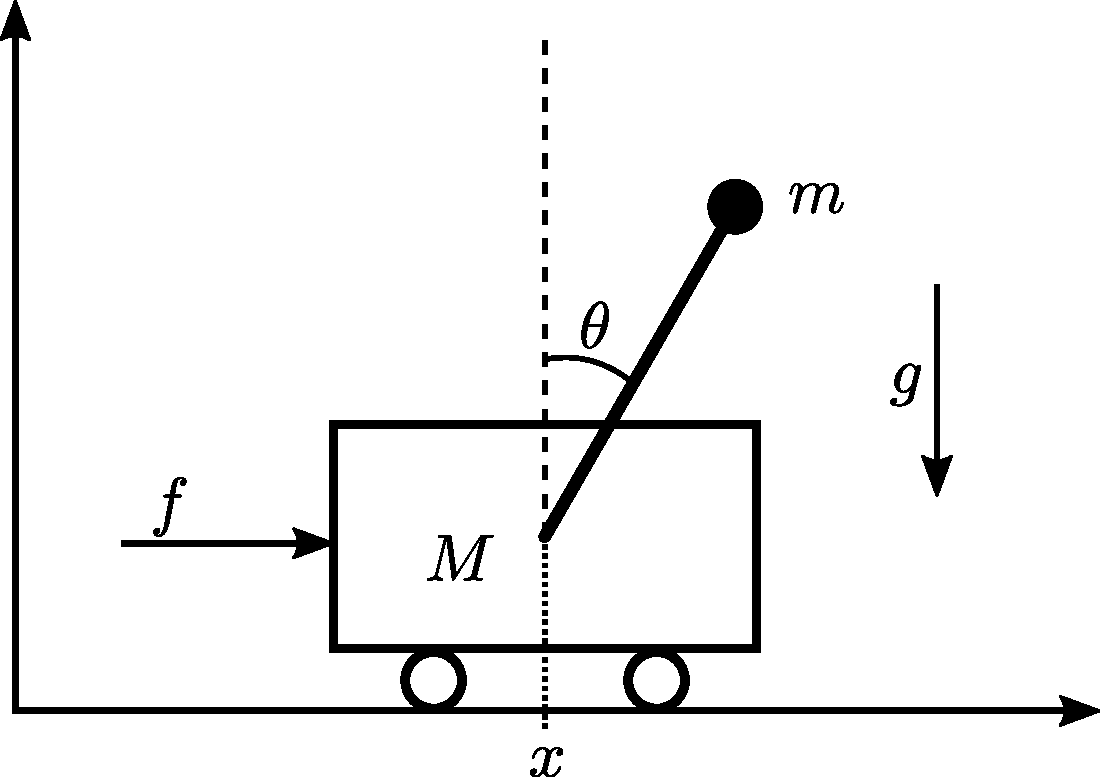
\includegraphics[width=.4\textwidth]{figures/system}
%  \caption{The cart pendulum system with generalized coordinates, $x$ and $\theta$, where $x$ is the center position of the cart, $\theta$ is the angle of the pendulum, $m$ is the point mass of the pendulum, $M$ is the mass of the cart, g is the gravitational acceleration and f is the force of actuation.}
%  \label{fig:system}
%\end{figure}

The system is presented with a specific task, see \autoref{fig:systemTask}. This aids in understanding the convinience of the presented trajectory planning tools, as the task requires nonlinear operation, where linearization alone is not enough.

\begin{figure}[H]
  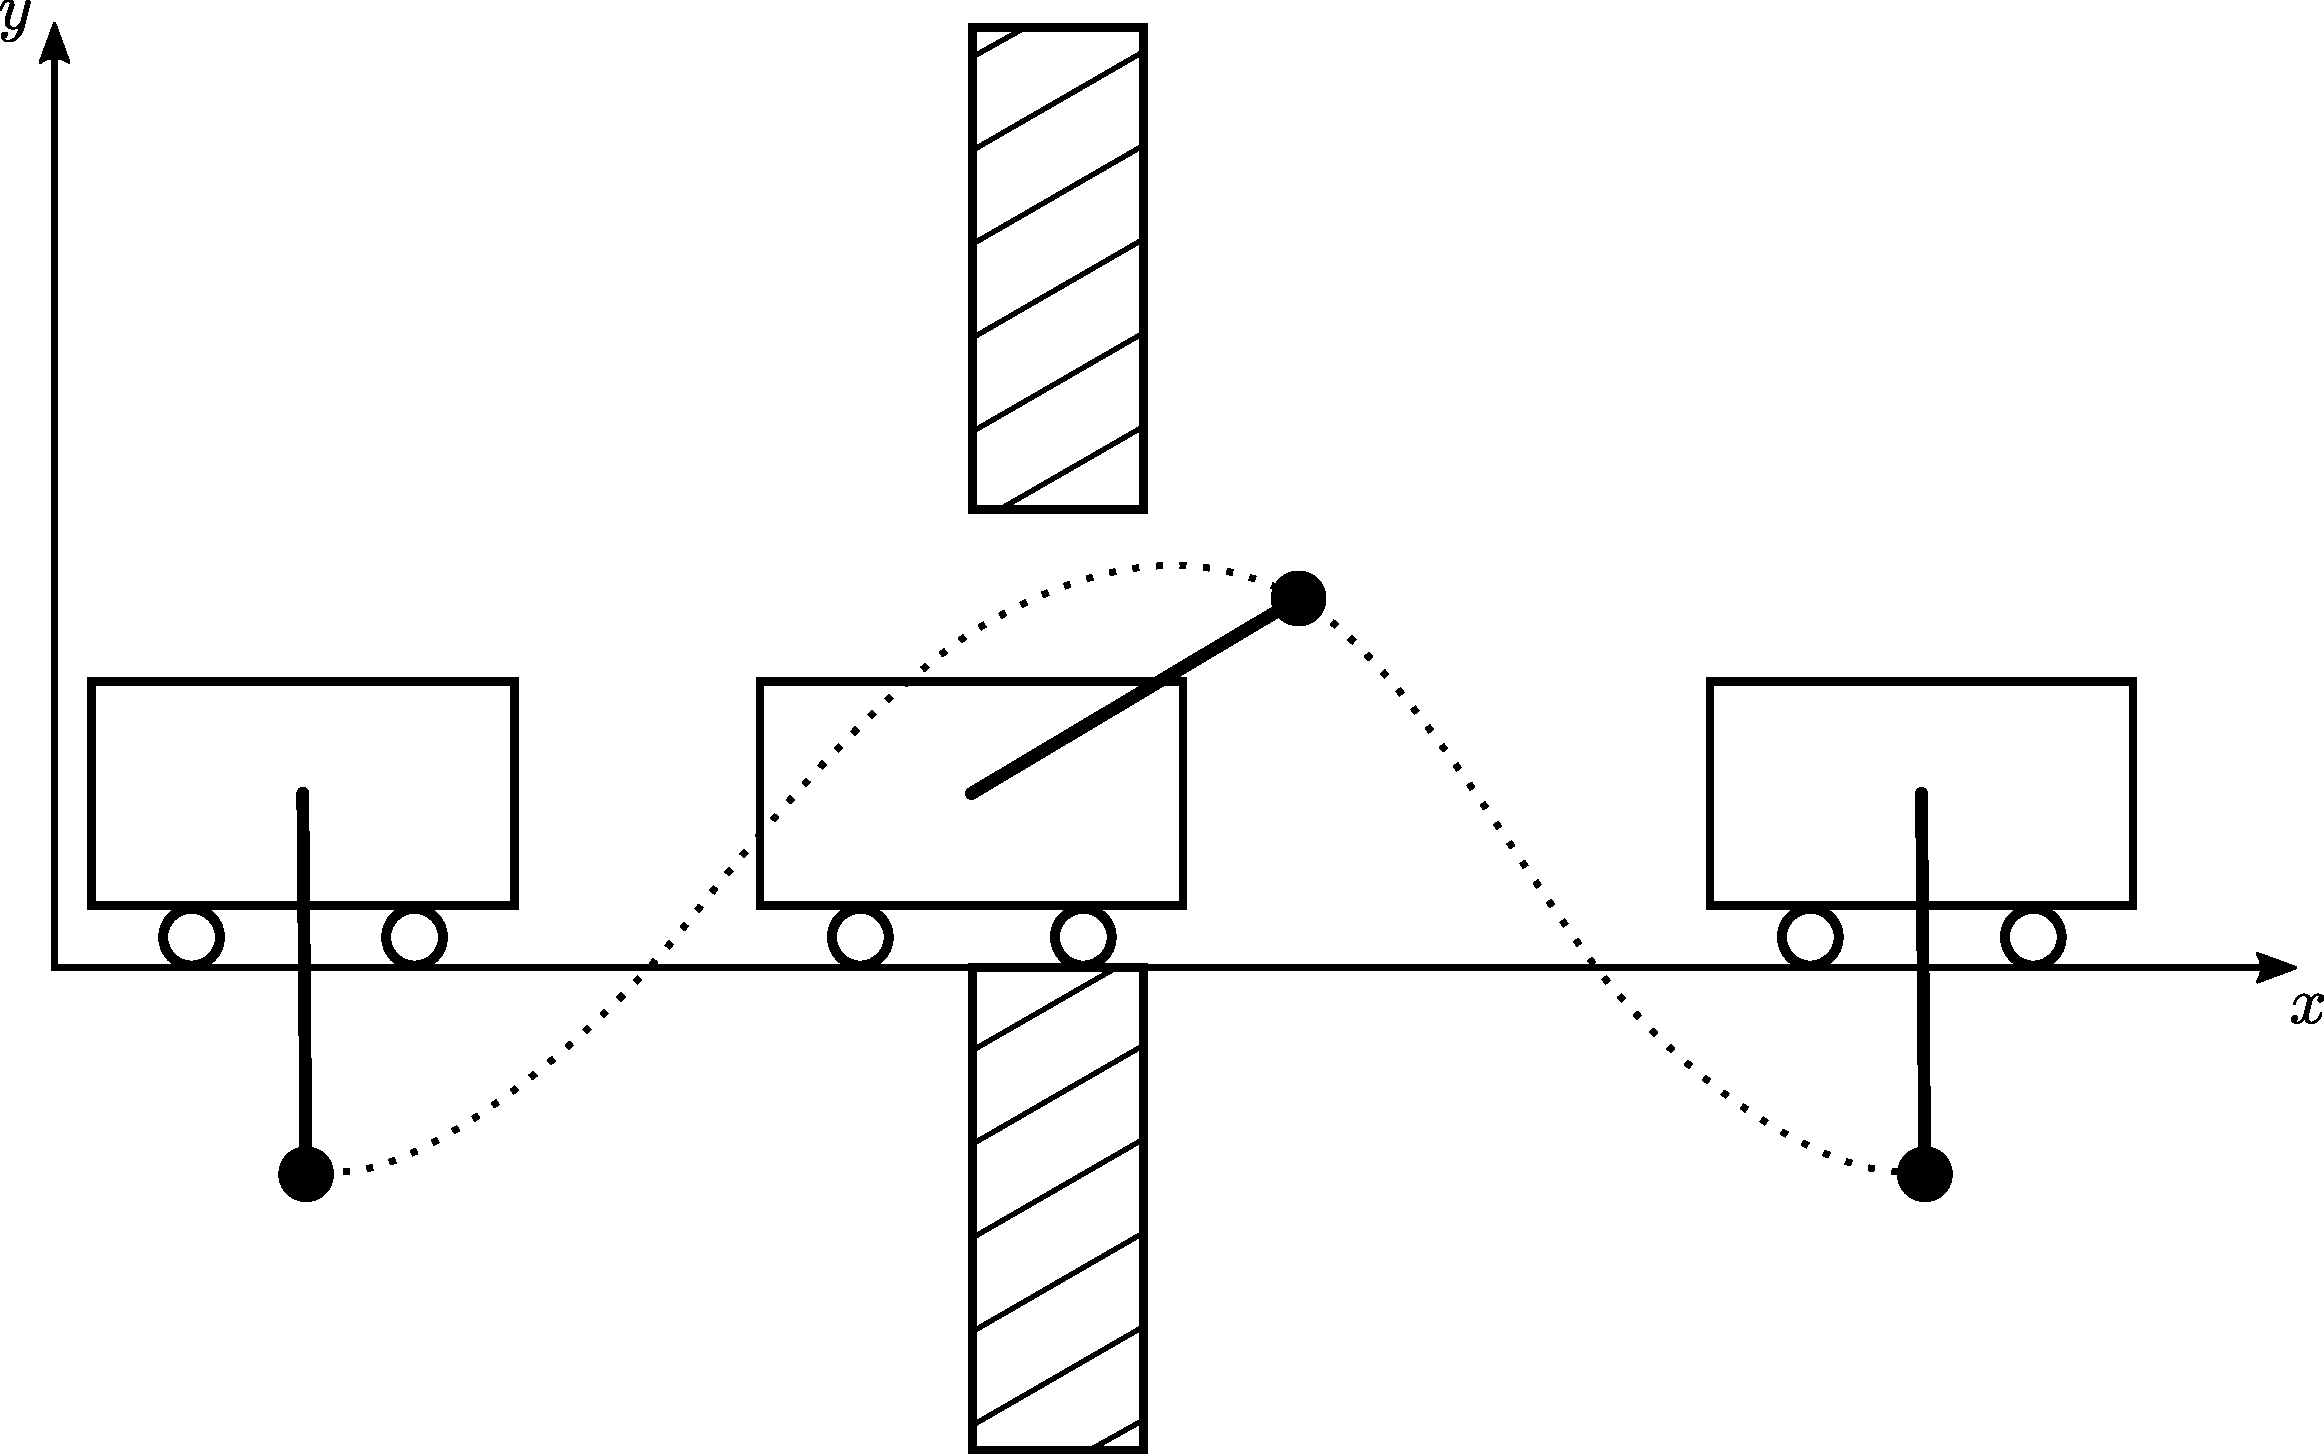
\includegraphics[width=.6\textwidth]{figures/systemTask}
  \caption{The task to be performed. The trajectory here is not realistic, and only shown to ilustrate the goal; avoiding the obstacles along the entire trajectory.}
  \label{fig:systemTask}
\end{figure}

